\chapter{Complementary physical datasets, dynamics and geometric inspection}
% Generated shared reviewed material.
\section{Complementary physical datasets and checked dynamics}
The learned program now has two additional, separately constructed corpora:
16,384 effective-material response records and22,951 molecular conformer/force
records in their default configurations. Time samples are not counted as
independent systems. Source-linked and dynamical configurations are additional.
The active HolonForge/Aster and Mora-3 repositories were read only; no data,
vocabulary, checkpoint, source enrollment or training process was changed.

The material corpus covers SSH, Kitaev, QWZ, Rice--Mele, Harper and actual
clean-dessin classical RG models. The molecular corpus includes designed
amides and peptides, with explicit-H MMFF94 calculations, geometric persistence,
and method-labelled conformations. Forty-eight existing Aster MP20 structures,
32 existing Mora PubChem identities and eight public PDB structures supply
separately labelled anchors. Their new computed responses are not new
experimental observations, DFT labels, binding affinities or CISS measurements.

All conformer, gauge, intervention and task descendants share a partition.
Specified physical/chemical similarity edges are closed transitively before
component-level stratification. Large components are kept intact even when
80/10/10 proportions or rare-class coverage become impossible. This gives a
finite, threshold-relative separation statement; it cannot guarantee every
kind of statistical independence or prevent overfitting. Source anchors are
train only. Molecular anchors are also checked against every default heldout
using the same chemical and applicable geometric thresholds; conflicting parent
groups are excluded. Global exposure to the models' previous corpora is a separate
evaluation gate.

For a number-conserving one-particle Hamiltonian $H$, write
$P_{ij}=\langle c_j^\dagger c_i\rangle$ and $U(t)=e^{-itH}$.
The data use $P(t)=U(t)P(0)U(t)^*$, occupations $n_i=P_{ii}$ and
outgoing currents $J_{ij}=-2\operatorname{Im}(H_{ij}P_{ji})$.
Then $\dot n_i=-\sum_jJ_{ij}$, directly from $i\dot P=[H,P]$.
Paired BdG evolution includes its independently computed condensate source;
it is not falsely treated as electron-number-conserving normal transport.
An exact interacting Hubbard dimer supplements Gaussian exchange correlations.
Molecular nuclear dynamics uses MMFF94, with a separately labelled,
uncalibrated effective $\pi$-orbital model for charge modulation.

Parquet configurations retain condition, target and evaluation roles, source
versions/hashes, units, failures and audit evidence. The local
\href{http://127.0.0.1:8765/datasets.html}{dataset explorer} shows actual
structures, currents, time evolution, graph wavelets and checked circuit
compilations. These computations support candidate discovery and model
validation; the independent arithmetic determinant/zero-location bridge remains
open. No new whole-chapter Lean formalization is asserted.

% Generated shared reviewed material.
\section{Construction, curation and interpretation}
\subsection{A record is an evidence-bearing physical task}
Each default Parquet row has a persistent record identity, parent/similarity
group, partition, evidence class, lossless scientific payload and typed numeric
columns. Forward inputs have the prefix \texttt{condition\_}; supervision uses
\texttt{target\_}; \texttt{evaluation\_} fields are excluded from inputs.
The full payload, source hash, record identifier and audit text are not
automatically fed into a model. Otherwise an apparent condition/target mask
could still leak the target through metadata or a duplicated representation.
An inverse task needs an explicit desired-condition contract and role change.

The origin fields distinguish a new simulation from a reused planned-source
identity or geometry with new labels. The source-anchor configuration preserves
existing train assignments. New public PDB coordinates retain their own source
identity rather than being called members of PDBbind or newly acquired
experimental quantum measurements. All anchors are train only: they do not
establish blind performance on a model that may have encountered the parent.

The actual native interfaces are tested without changing either model.
Aster accepts condition-only Hamiltonian records through its existing tokenizer.
Changing a hidden target leaves those input tokens unchanged. Mora-3's scalar
graphs preserve computed/predicted evidence. Its existing scalar/array
supervision interfaces reject those targets under their observed-only policy.
That rejection is recorded, not bypassed by changing the evidence label.
Source construction is therefore distinct from the owning model's future
admission, scaling, objective and evaluation decisions.

\subsection{Effective material families and gap guards}
The two-band QWZ model uses
\[
 H(k_x,k_y)=\sin k_x\,\sigma_x+\sin k_y\,\sigma_y
 +(m+\cos k_x+\cos k_y)\sigma_z.
\]
Its continuum band gap is
$2\min\{|m+2|,|m|,|m-2|\}$. To see this, put
$u=\cos k_x$, $v=\cos k_y$. The squared positive energy is
$2+m^2+2m(u+v)+2uv$, a bilinear function on $[-1,1]^2$;
its minimum occurs at a corner. Thus an odd mesh that misses $\pi$ cannot
certify a gap near $m=0$ or2. The corrected release uses this analytic guard,
even32/64 meshes, random gauge checks and an unavailable label near closure.
The occupied-band integer uses the oriented link-product convention of
Fukui--Hatsugai--Suzuki \cite{DSFHS}; the sign convention is retained in the row.

For the Rice--Mele pump, take
$t_1=1+\delta\cos\theta$, $t_2=1-\delta\cos\theta$ and
$\Delta=r\sin\theta$. With positive $t_1,t_2$, minimization over $k$ first
gives $(t_1-t_2)^2+\Delta^2$ at $k=\pi$; minimization over $\theta$ gives
the exact gap $2\min(2\delta,r)$. Harper's direct gap has a conservative
mesh/Lipschitz guard, explicitly distinguished from interval certification.
The displayed bulk slice has $k_y=0$; an open strip is evaluated separately at
$k_y=.37$. A single strip is not a proof of its entire edge dispersion.

The SSH winding, Kitaev sign invariant and classical dessin RG retain their
own hypotheses. Surface genus is not an electronic phase index. In the
Kitaev row, a physical onsite defect changes particle and hole diagonals with
opposite signs. Its gauge change has the form $\operatorname{diag}(G,\bar G)$.
These preserve the recorded particle--hole symmetry; arbitrary independent
diagonal perturbations would not. A quarantined draft revealed this error
before release. No failed draft replaces a verified artifact.

\subsection{Molecular geometry and forces}
The molecular set contains explicit chemical graphs, atom order, hydrogens,
stereochemistry, method-labelled optimized references and bounded coordinate
perturbations. MMFF94 supplies empirical molecular-mechanics energies, analytic
forces and partial charges \cite{DSRDKit}. It supplies neither ab-initio
electron density nor experimental affinity, ADMET, redox or biological efficacy.
An optimization convergence code is not a theorem of a unique global minimum.
Absolute MMFF energies are not cross-molecule atomization energies.

The checker reconstructs the stored bond graph in its \emph{actual atom order}.
A canonical SMILES string determines chemical identity but need not give the
coordinate-array order. Geometry-assigned stereochemistry is checked against
that identity; mirror controls fail. Energies and forces are recalculated on
every accepted record. Central energy differences check force signs/units,
and proper rotations/translations check the expected scalar/vector behavior.
Missing or unsupported labels are not imputed.

For the heavy-atom point cloud, the complete finite Vietoris--Rips2-skeleton
gives $H_0,H_1$ over $\mathbb F_2$. All edges and triangles, including ties,
are ordered explicitly. Independent boundary-rank calculations verify selected
Betti numbers against the barcodes. These are geometric distance-filtration
features; a molecular loop or persistence bar is not an electronic topological
phase. MMFF and the idealized $\pi$-orbital Hamiltonian retain separate labels.

\subsection{What the split certificate proves}
Let $V$ be the finite parent set and connect two parents whenever a declared
similarity test passes. Add edges for all shared source/variant lineages.
Assign a partition to each connected component and inherit it for every row.
If an accepted similarity edge joined two partitions, its endpoints would lie
in one component with two assignments, a contradiction. This proves the exact
finite no-crossing property for the declared relation.

For materials, normalized parameter and relative finite-spectrum thresholds
are family/size-specific. SSH hopping swaps, Kitaev chemical-potential sign
and the classical RG global-sign symmetry are folded conservatively. For
molecules, stereo-agnostic constitution, nonempty Murcko scaffold and
radius-two Morgan Tanimoto threshold $.65$ form chemical components. A second
all-conformer pass adds edges for equal heavy-element multisets with sorted
pair-distance RMS at most $.10$\AA. This descriptor is rotation/permutation
invariant but is not a complete congruence invariant or a certified RMSD
optimizer; conservative false-positive grouping is possible.

Whole-component allocation balances row counts and declared family/topology
or molecular-size/persistence strata. It never breaks a component to manufacture
an80/10/10 result. The large peptide component makes the molecular training
partition much larger than80\%; rare/held-out peptide coverage can consequently
be absent. Exact distributions and cross-partition nearest witnesses accompany
the release. Protein TM-score, homology separation and global overlap with the
models' complete historical corpora are not certified by small-molecule
fingerprints. Threshold separation cannot itself guarantee freedom from all
leakage or overfitting.

\subsection{Motion, charge modulation and exchange}
For normal free fermions, $P(t)=UP(0)U^*$ preserves Hermiticity, trace and the
spectrum: $P^*=P$ follows by adjoints, trace follows by cyclicity, and
$P(t)=U P(0)U^{-1}$ is a similarity. Thus $0\leq P\leq I$ and projector
occupancy remain valid. Computing the diagonal of $-i[H,P]$ gives
\[
 \dot n_i=2\operatorname{Im}\sum_jH_{ij}P_{ji},\qquad
 J_{ij}=-2\operatorname{Im}(H_{ij}P_{ji})=-J_{ji}.
\]
The currents therefore obey site continuity and conserve total particle number.
Their arrows represent probability/particle flux, not measured trajectories of
individual electrons. Charge modulation is $-[n_i(t)-n_i(0)]$ in the declared
electron-charge convention.

For a paired model, put $\Psi=(c,c^\dagger)$ and
$R=\langle\Psi\Psi^\dagger\rangle$. From an initial Slater projector use
$R_0=\operatorname{diag}(I-P_0,P_0^{\mathsf T})$. Evolve with the full BdG
Hamiltonian and recover $P=I-R_{11}$, $F=R_{12}$.
The independently computed pairing source is
\[
 S_i=-2\operatorname{Im}(\Delta F^*)_{ii},\qquad
 \dot n_i=-\sum_jJ_{ij}+S_i.
\]
The commutator derivative and this separate source formula agree in the
checks; the source is not defined as the residual of the desired equation.
For a Gaussian state, Wick's rule gives, for $i\ne j$,
$\operatorname{Cov}(n_i,n_j)=|F_{ij}|^2-|P_{ij}|^2$; on the diagonal it is
$n_i(1-n_i)$. The negative term is an exchange hole, not a computed Coulomb
exchange-energy functional. Explicit small Fock-space evolution independently
checks the covariance, current and pairing conventions.

The interacting control is the two-site Hubbard model at two electrons:
\[
 H=-t\sum_\sigma(c_{0\sigma}^\dagger c_{1\sigma}+\mathrm{h.c.})
   +U\sum_{a=0}^1n_{a\uparrow}n_{a\downarrow}.
\]
In its singlet/doubly-occupied symmetric sector the matrix is
$\left(\begin{smallmatrix}0&-2t\\-2t&U\end{smallmatrix}\right)$;
the triplet energy is zero. Diagonalizing gives the exact exchange gap
$J=(\sqrt{U^2+16t^2}-U)/2$, approaching $4t^2/U$ for large positive $U$.
The full six-state two-electron sector supplies density, spin-swap and current
trajectories; a separate16-state Jordan--Wigner calculation checks them.
This finite dimer is not a thermodynamic phase classification.

For nuclei, velocity Verlet uses actual MMFF forces and masses, with explicit
time/energy units, finite energy drift and momentum checks. A Grad-only RDKit
loop initially reused stale distance information. Refreshing energy at the same
coordinates before the gradient restored the expected second-order step-size
behavior in independent refinement tests. Failed trajectories are retained and
excluded. The finite isolated trajectories are not equilibrium sampling.
MMFF charges remain fixed. The separate uncalibrated $\pi$ graph has its own
dimensionless electronic time; it is not self-consistent TDDFT coupled to the
nuclear femtosecond trajectory.

\subsection{Source-backed peptides and genuine boundaries}
Public wwPDB coordinates are supplied under CC0 \cite{DSPDB}. The source packet
includes Trp-cage1L2Y, villin1VII, historical Trp-zipper1HRW (superseded by
1LE0, with the actual file HEADER identity retained), pancreatic polypeptide1PPT,
azurin1AZU, crambin1CRN, ubiquitin1UBQ and engrailed homeodomain1ENH.
The full source file, checksum, DOI, first-model/chain selection and bounded
residue-subsystem mapping remain explicit. An NMR ensemble's model order is
not physical time. Azurin's electron-transport classification does not calibrate
our coarse contact Hamiltonian or turn it into an electronic-structure result.

The CISS review and peptide-bridge charge-transfer preprint motivate future
spin, environment and lead benchmarks \cite{DSCISS,DSBridge}; the source review is
focused, not an independent reproduction of their experiments. A spinless
contact graph cannot supply their spin polarization, electron-transfer rates
or measured quantum-biological mechanism. Synthetic strain, vacancy, mirror,
coupling and conformer variants have their own provenance and share the parent
group. They are additional training candidates, not newly observed systems.

\subsection{Circuits and geometric visualization}
For a normal one-particle unitary $U$, adjacent row elimination gives Givens
matrices $G_k$ and diagonal phases $D$ with
$U=G_1^*\cdots G_m^*D$. For $a,b$ in one column, the eliminating block is
\[
 G=\frac1{\sqrt{|a|^2+|b|^2}}
 \begin{pmatrix}\bar a&\bar b\\-b&a\end{pmatrix}.
\]
Direct multiplication gives $G(a,b)^{\mathsf T}=(r,0)^{\mathsf T}$ and
$G^*G=I$. A two-mode second-quantized gate acts as $1$ on the vacuum, as its
one-particle block on the single-occupation sector and as the determinant on
double occupation. The exported circuit verifies these matchgates and numerical
recomposition. Browser replay applies the actual gates to the saved initial
correlation matrix. BdG pairing needs a different Bogoliubov compiler; it is
not passed by a number-conserving Givens circuit. The Hubbard example instead
includes Jordan--Wigner parity and measured product-formula convergence.

Actual molecular structures use CPK colors and explicit atom/bond order, with
SDF/XYZ views, ball-and-stick, sticks and space-filling representations.
Effective material-site layouts are labelled schematic. Electron-colored
Gaussian splats are declared kernels on discrete site values, not ab-initio
volumetric density. For the symmetric graph Laplacian $L$, localized wavelets
are $sLe^{-sL}\delta_i$; since $\mathbf1^{\mathsf T}L=0$, they have zero sum.
Their signed colors are not probabilities. Time as a fourth projection
coordinate is a visualization operation, not a new spatial dimension.

The dataset page links the checked public releases and source code. The full
new probabilistic/homological/physical interfaces are not yet packaged in Lean;
the existing $360$ printed reports retain their earlier scope. Neither a simulated
transport law, dataset split certificate nor a compiled finite circuit closes
the arithmetic comparison required for GRH.

\begin{figure}[htbp]
\centering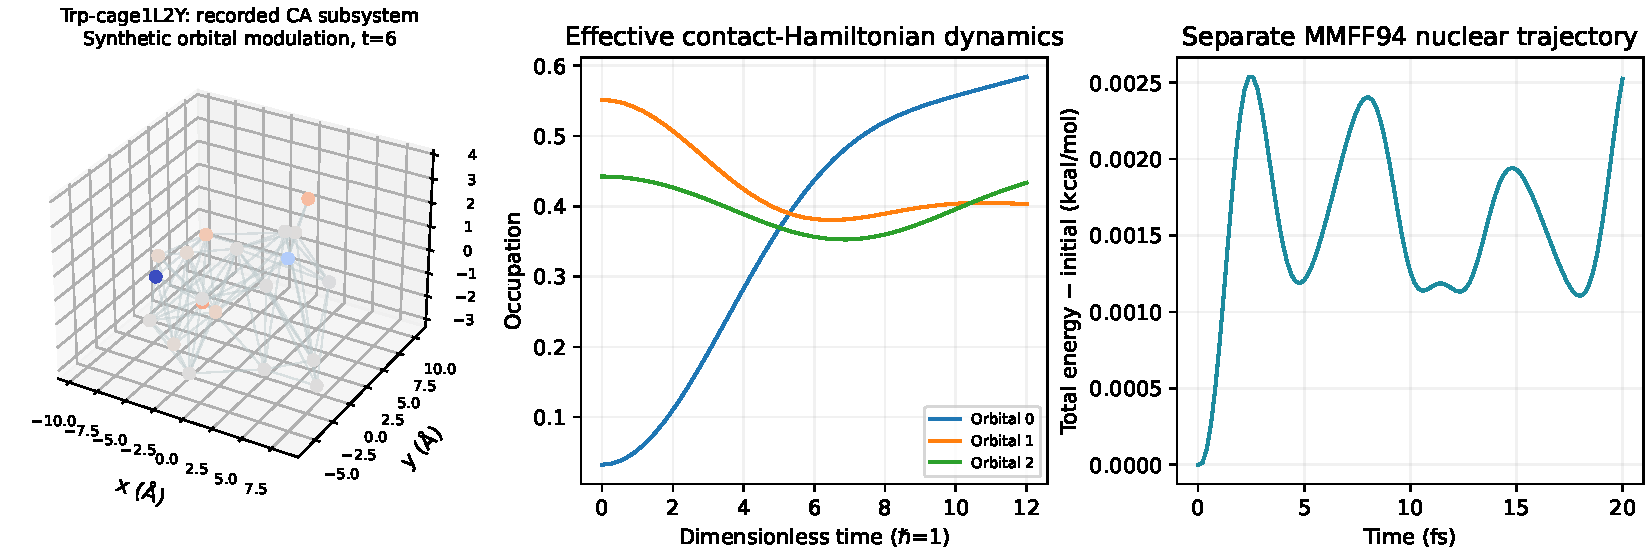
\includegraphics[width=\textwidth]{figures/complementary-datasets.pdf}
\caption{Actual source-backed and computed examples. Left: the recorded Trp-cage
CA subsystem, colored by an uncalibrated contact-model orbital modulation.
Middle: three of its finite orbital occupations. Right: total-energy drift of a
separate explicit-H MMFF94 trajectory. Electronic time and nuclear femtoseconds
are distinct; the contact model is neither an experimental transfer rate nor
an ab-initio density. The interactive tool supplies the actual records and code.}
\end{figure}
\begin{figure}[htbp]
\centering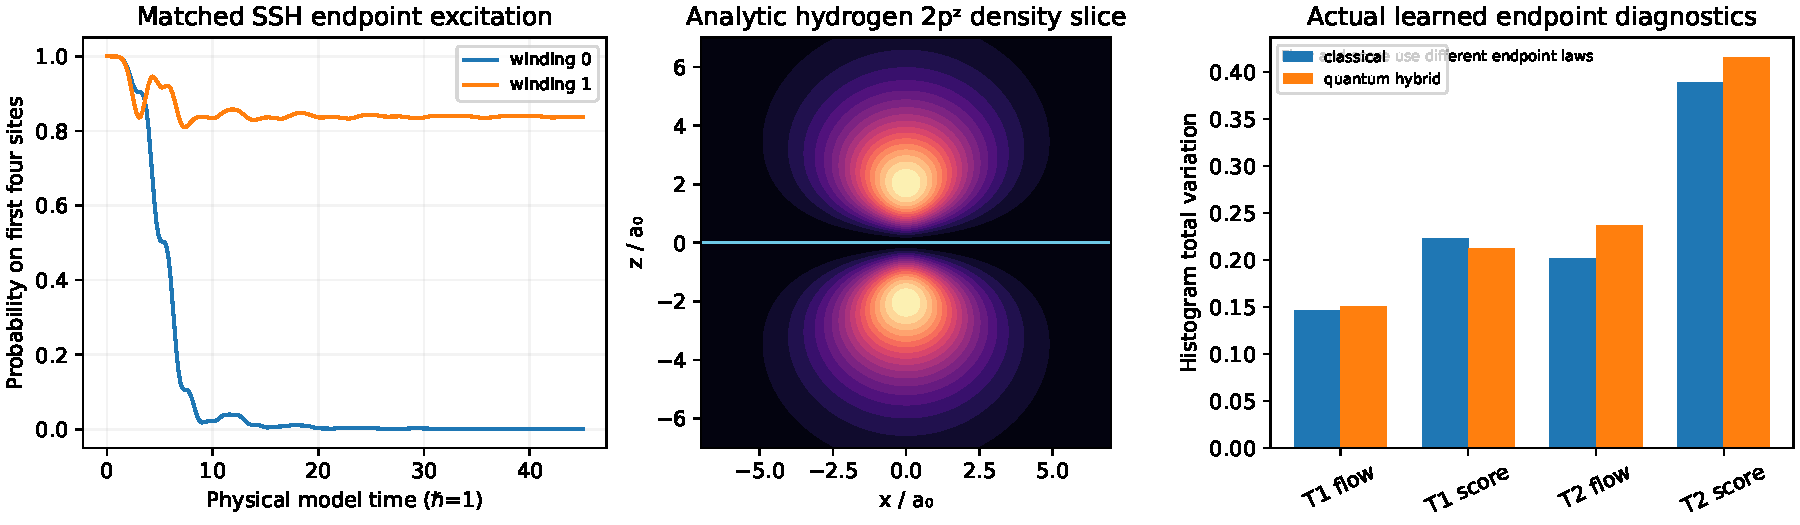
\includegraphics[width=\textwidth]{figures/orbital-flow.pdf}
\caption{Computed matched SSH transport, an analytic hydrogen orbital slice and actual trained chemistry endpoint diagnostics. The diffusion endpoint retains positive heat time; its reference differs from the flow target. These finite results do not establish quantum advantage.}
\end{figure}
\begin{figure}[htbp]
\centering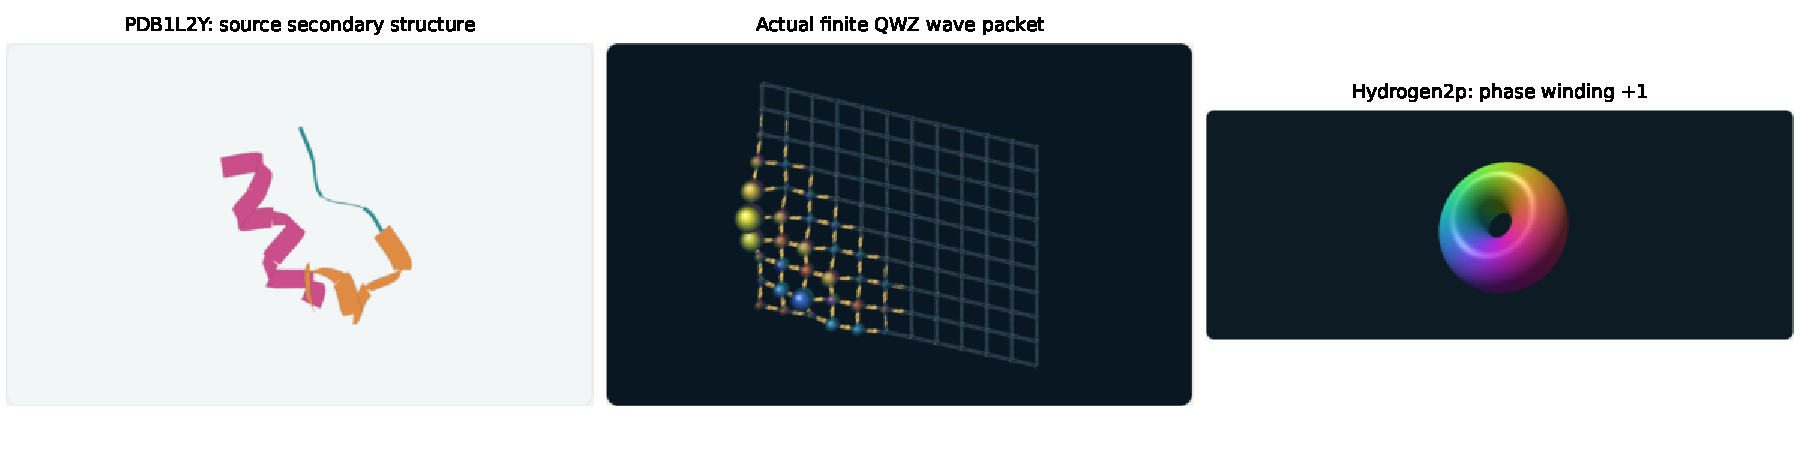
\includegraphics[width=\textwidth]{figures/orbital-atlas.pdf}
\caption{Native interactive renderings: deposited Trp-cage secondary structure, an actual finite QWZ wave packet and an analytic hydrogen phase vortex. Ribbon, probability-height and density-isosurface encodings have different source and physical meanings.}
\end{figure}
% Generated shared reviewed material.
\section{Molecular structure, complex transport and learned chemistry}
The complementary-data laboratory now separates deposited protein structure,
actual finite quantum transport and learned conformation generation. Covalent
bonds use explicit molecular graphs or qualified PDB templates, with depth
ordering and visible atom/bond scales. The ribbon view reads deposited
\texttt{HELIX}/\texttt{SHEET} records; short synthetic peptide backbones remain
unassigned rather than acquiring invented secondary structure.

Five additional finite propagation examples compare matched SSH/QWZ
topological and trivial controls and an SSH domain wall. Complex phase,
probability, current, coherence and selected eigenstates are distinct views.
Analytic hydrogen volumes illustrate nodes, quantum beats and a phase vortex;
they are not molecular electronic-structure calculations. Eight further CPU
runs train classical and two-qubit hybrid score/flow models on periodic MMFF
butane/pentane torsion spaces. All checkpoints, losses, controls and positive
noise endpoints are explicit. These examples neither establish quantum
advantage nor close the independent arithmetic bridge for GRH.

% Generated shared reviewed material.
\section{Geometry, orbitals and generative time}
\subsection{Chemical connectivity and source secondary structure}
An atomic coordinate cloud does not determine chemical bonds merely by
looking connected. SDF graphs retain their explicit bond indices. For the PDB
source view we select the first model, blank/A alternate locations and positive
occupancy; solvent is omitted from the display. Standard amino-acid templates,
explicit \texttt{CONECT}, qualified ligand/hydrogen proximity and geometrically
valid peptide C--N links have separate provenance. The complete original file
remains available. Display connectivity is not a newly measured bond label.

The parser follows the wwPDB3.3 record definitions \cite{VisPDB}. A class-one
\texttt{HELIX} is an alpha helix; class five is a $3_{10}$ helix, not another
alpha helix. \texttt{SHEET} retains strand identity, sheet membership and
parallel/antiparallel sense. Ribbon patches follow the actual CA trace and
carbonyl orientation, with strand arrows and narrower coils. A peptide bond
must connect neighboring residues before a patch or spline-control neighbor
is allowed: spatially nearby disconnected fragments and TER-separated chains
must not acquire a phantom ribbon. Regression tests include these controls.
Backbone recognition in a short synthetic SDF peptide supplies a trace, not a
DSSP assignment or evidence of a stable secondary structure.

The full-source geometry is distinct from the capped effective contact graph.
In the full-source view, only mapped modeled CA sites carry its electronic
field. Nuclear display interpolation adds no new integration steps. An NMR
model index, a ribbon parameter and a generative time are not physical time.

\subsection{What the complex transport animation computes}
For a finite Hermitian matrix $H=V\operatorname{diag}(E_k)V^*$ and a normalized
initial vector $\psi_0$, the continuously evaluated browser state is
\[
 \psi_j(t)=\sum_k V_{jk}e^{-itE_k}(V^*\psi_0)_k.
\]
Unitarity gives $\sum_j|\psi_j(t)|^2=1$. Differentiating gives
$\dot n_i=2\operatorname{Im}\sum_jH_{ij}\psi_j\bar\psi_i$ and hence
$\dot n_i+\sum_jJ_{ij}=0$ for
$J_{ij}=-2\operatorname{Im}(H_{ij}\psi_j\bar\psi_i)$.
The actual complex one-particle coherence is
$\rho_{ij}=\psi_i\bar\psi_j$. A common phase cancels from both current and
coherence; node colors therefore use a stated phase reference. The probability
height is a display encoding, not another physical coordinate. Current arrows
are fluxes, not classical electron paths.

Two48-site SSH controls use the same initial endpoint orbital and exchanged
strong/weak hoppings. Their periodic bulk winding is respectively zero and
one for $q(k)=t_1+t_2e^{ik}$, with gap $2|t_1-t_2|$. A separate61-site domain-wall chain starts and ends
with strong bonds and has two weak bonds adjacent to its central even site.
Its sublattices have sizes31 and30. At zero energy, set the odd-site amplitudes
to zero and solve the tridiagonal recurrence on even sites. The amplitudes
decay away from the wall by the weak/strong ratio. The nonzero off-diagonal
entries determine this vector up to scale, so the nullspace is one-dimensional.
This proves a finite interface zero mode; it does not identify an arithmetic
Hilbert--P\'olya spectrum.

The QWZ examples have a $12\times10$ rectangle and two orbitals per site.
They use the same unfiltered corner spinor for masses $-1$ and $-3$.
Their bulk Chern numbers are $-1$ and0 in the existing link-product convention;
32/64 meshes and gauge controls agree. Finite boundary probability, spectral
weights and coherence remain measurements of the particular finite state,
not definitions or proofs of that bulk invariant. Independent matrix-exponential
checks reproduce the five propagated states. The hydrogen phase winding below,
chemical torsion torus, dessin genus and persistent-homology classes are also
different invariants.

\subsection{An analytic orbital benchmark with actual nodes}
In atomic units, take $h=-\frac12\Delta-r^{-1}$ on the usual hydrogen domain.
The displayed normalized eigenfunctions are
\[
 \phi_{1s}=\pi^{-1/2}e^{-r},\qquad
 \phi_{2s}=\frac{(2-r)e^{-r/2}}{4\sqrt{2\pi}},\qquad
 \phi_{2p_j}=\frac{x_j e^{-r/2}}{4\sqrt{2\pi}}.
\]
Their energies are $E_1=-1/2$, $E_2=-1/8$. The angular integrals and
$\int_0^\infty r^n e^{-ar}\,dr=n!a^{-n-1}$ give their unit norms;
opposite angular parity gives orthogonality of $1s$ and $2p_z$.
Consequently
\[
 \psi(t)=\sqrt{1-a}\,\phi_{1s}
       +\sqrt a\,e^{-3it/8}\phi_{2p_z},\qquad 0\le a\le1,
\]
has unit norm after removing its unobservable common ground-state phase.
Its density has the interference term
$2\sqrt{a(1-a)}\phi_{1s}\phi_{2p_z}\cos(3t/8)$: this is the actual quantum
beat shown in the volume. The $2s$ radial node is $r=2$; the $2p_z$ nodal
plane is $z=0$.

The state $(\phi_{2p_x}+i\phi_{2p_y})/\sqrt2$ is proportional to
$(x+iy)e^{-r/2}$. On a circle avoiding the nodal axis its phase winds once,
and $L_z\psi=\psi$. Its current is
$\operatorname{Im}(\bar\psi\nabla\psi)$ and has an azimuthal component.
This stationary density with nonzero current need not show a moving classical
particle. A finite-radius ray-marched volume and its opacity/exposure curve
are rendering choices, distinct from the analytic density and normalization.
These are nonrelativistic isolated-hydrogen benchmarks, not many-electron
molecular orbitals or ab-initio peptide density.

\subsection{A useful periodic chemical target}
Butane has one selected torsion; pentane has two. All other internal coordinates
are held at the recorded MMFF reference geometry. The finite grids have72 and
$24^2$ points, respectively. At300K define
\[
 p_k=Z^{-1}\exp[-(E_k-E_{\min})/(k_BT)],\qquad
 q_0(\theta)=\sum_k p_k\,K_{\sigma^2/2}(\theta-\theta_k),\quad \sigma=.05,
\]
where the product wrapped heat kernel is used on $\mathbb T^d$ and $d=1,2$.
Thus $q_0$ is an explicitly softened finite-grid Gibbs target. It is positive,
smooth and normalized; it is not a full solvent or molecular-equilibrium
distribution. No affinity, redox, efficacy or electronic-density label is inferred.
The molecular animation rotates downstream atoms about each actual bond axis;
its poses agree with independent RDKit dihedral assignments to numerical
precision and preserve the bond graph and fixed bond lengths.

\subsection{Score diffusion on the torus}
For the unit circle,
\[
 K_\tau(x)=\sum_{m\in\mathbb Z}\frac{e^{-(x+2\pi m)^2/(4\tau)}}{\sqrt{4\pi\tau}},
 \qquad \partial_\tau K_\tau=\partial_x^2K_\tau.
\]
The product kernel gives $q_\tau=q_0*K_\tau$ and
$\partial_\tau q_\tau=\Delta q_\tau$. A forward sample is
$X_\tau=\operatorname{wrap}(X_0+\sqrt{2\tau}\,\xi)$.
Conditioning the wrapped Gaussian mixture shows
\[
 \nabla\log q_\tau(x)
 =\mathbb E[-\xi/\sqrt{2\tau}\mid X_\tau=x].
\]
Indeed, differentiate each image term and divide by the mixture density;
the Gaussian score is the stated latent-noise target. Conditional least
squares therefore identifies the marginal score. The implemented weighted
DSM loss uses weight $2\tau$, not an unlabelled Euclidean proxy on cut angles.
The periodic-input network is trained over the full normalized time interval.

With reverse clock $u$, the ideal SDE is
$dY_u=2\nabla\log q_{T-u}(Y_u)\,du+\sqrt2\,dW_u$.
Its Fokker--Planck equation at density $q_{T-u}$ is
$-2\Delta q+\Delta q=-\Delta q$, as required. This connection to score SDEs
is the standard method \cite{VisScore}; the periodic mixture here supplies an
explicit control. Initialization is sampled from the actual $q_T$, with $T=2$,
rather than silently assuming it is uniform. Sampling stops at $\tau=.03$,
so the ideal endpoint is $q_{.03}$, whose Gaussian component variance is
$\sigma^2+.06$. It is not $q_0$. The initial run exposed this distinction;
its source and outputs are preserved. The corrected run uses the proper endpoint
reference and no excluded small-time training interval.

Exact wrapped-mixture scores, finite-difference checks, nested64/128-step
Brownian controls and stored learned trajectories accompany the experiment.
A finite Euler diagnostic is neither a convergence theorem nor a guarantee
that a learned score recovers equilibrium. Remaining noise and learned-field
error are shown separately from the MMFF target.

\subsection{Wrapped-geodesic flow matching}
Let $X_0$ be uniform on $\mathbb T^d$, independently let $X_1\sim q_0$, put
$D=\operatorname{wrap}(X_1-X_0)$ and
$X_t=\operatorname{wrap}(X_0+tD)$. The cut locus has probability zero under
these continuous laws. For every smooth periodic test function $f$,
\[
 \frac d{dt}\mathbb Ef(X_t)
 =\mathbb E\langle\nabla f(X_t),D\rangle
 =\int\langle\nabla f(x),v_t(x)\rangle\rho_t(x)\,dx,
 \quad v_t(x)=\mathbb E[D\mid X_t=x].
\]
This is the weak continuity equation with the correct uniform and $q_0$
endpoints. Writing $B=[-\pi,\pi]^d$, the conditional formulas are explicitly
\[
 \begin{aligned}
 \rho_t(x)&=(2\pi)^{-d}\int_Bq_0(x+(1-t)D)\,dD,\\
 \rho_t(x)v_t(x)&=(2\pi)^{-d}\int_BD\,q_0(x+(1-t)D)\,dD.
 \end{aligned}
\]
Because $q_0$ is smooth and strictly positive on the compact torus,
these integrals are jointly smooth through both endpoints and
$\rho_t\ge\min q_0>0$. Division gives a smooth bounded periodic $v_t$
with a uniform spatial Lipschitz bound. In particular $v_1=0$ by symmetry. The usual unique flow of this globally Lipschitz
time-dependent field transports the stated marginals. Conditional regression
targets $D$ and learns an approximation to $v_t$, following the flow-matching
and manifold formulation \cite{VisFlow,VisRFM}. Neither the regression loss
nor a visualization replaces endpoint-error measurement.

\subsection{Physical state preparation, RG and phase-conditioned design}
The earlier seven-spin dessin experiment supplies an actual quantum Gibbs
state and its partial trace; its learned circuits approximate specified
state/field targets. The exact coarse action in the RG chapter is produced
by integrating out physical spins. Here the chemical learner transports a
classical probability law on internal coordinates. A quantum channel, an RG
partial trace and a score/noise schedule are three different constructions,
with different states, clocks and acceptance tests.

A concrete materials-design constraint already appears in the QWZ controls.
Any continuous mass path from $m=-3$ to $m=-1$ passes through $m=-2$.
The explicit bulk gap formula then gives zero gap. Thus such a generator
cannot both change between these two Chern sectors and preserve the gap
throughout that path. Sector-conditioned sampling, explicit transition
states and gap/invariant checks are meaningful design tasks. Merely drawing
a continuous latent interpolation does not meet them. The finite transport
controls and the earlier learned thermal-state experiments provide distinct
physics benchmarks for these requirements, rather than unverified
predictions of a synthesized topological material.

\subsection{What the quantum hybrid actually contributes}
Each hybrid has two re-uploading two-qubit layers: periodic $R_z$ angle/time
encoding, trainable $R_y$ rotations and CZ, followed by eight actual Pauli
expectations and a two-layer64-unit tanh classical readout. The angles and
readout are trained together. Integer coordinate frequencies preserve
$2\pi$ periodicity of the measured features, and composition preserves it in
the vector field. These are classically simulated quantum-feature hybrids,
not coherent quantum chemical evolution or quantum-assisted measurements.
The matched classical controls use periodic first/second harmonics and the
same readout width. Parameter counts and individual seeds remain explicit.

Eight2400-update CPU runs retain heldout objectives, checkpoint weights,
periodicity errors, independent Kronecker/Pauli calculations, parameter
finite differences, exact-score comparisons and actual endpoint histograms.
The limited runs do not establish quantum advantage. Flow and diffusion have
different positive-noise endpoint laws and must not be ranked as though their
targets were identical. Generative interpolation time is not molecular time.

The chemical torus is a concrete internal-coordinate space. Drawing it next
to a dessin, a noncommutative torus or a Fukaya construction does not construct
a functor or prove homological mirror symmetry. Likewise none of these finite
learners constructs the missing arithmetic self-adjoint determinant bridge.
Adding heat/noise is also distinct from integrating out physical degrees of
freedom in the earlier actual RG chapter; a noise schedule alone is not an RG
construction. New source, operator-domain, arithmetic and Lean obligations remain explicit.

\IfFileExists{chapters/dataset-release-links.tex}{\section{Public release access}
Both datasets are additional public Parquet releases, with dataset cards,
origin columns, source records, audit evidence and exact remote hashes.
\paragraph{Aster complementary topological response}\href{https://huggingface.co/datasets/AmelieSchreiber/GRH-Aster-TopoResponse-20261104}{Public Hugging Face dataset}.\\
Default static rows: 16,384; separately labelled source-anchor rows: 576.\\
Verified dataset commit: \texttt{2b8ce36571298a3517b8c88bb23269341d9b8908}.\\
\paragraph{Mora complementary conformer response}\href{https://huggingface.co/datasets/AmelieSchreiber/GRH-Mora-ConformerResponse-20261104}{Public Hugging Face dataset}.\\
Default static rows: 22,951; separately labelled source-anchor rows: 266.\\
Verified dataset commit: \texttt{53a6b66acaa69ef79584648f3f6dc068363c4837}.\\
Use the pinned commit and configuration names from the dataset card; time
frames do not count as independent systems. The interactive explorer retains
the full release receipts and actual source-file downloads. No dataset was
enrolled into either active model during this work.

The data commits above remain immutable. Public visibility was enabled at the
owner's request on 4 November 2026, with new card-only commits recorded in
\texttt{outputs/publication/2026-11-04}. No data file changed.
}{}

% Generated shared reviewed material.
\section{Coherent electron-density clouds in an explicit spatial basis}
The density viewer now evolves spatial functions, including interference
terms, instead of drawing independent spheres around occupied sites. Let
$g_i(\mathbf r)$ be normalized real Gaussian basis functions, let
$S_{ij}=\int g_i g_j$ be their positive-definite overlap, and set
$L=S^{-1/2}$. For a Hermitian orthonormal-basis Hamiltonian $h$ and a matrix
$C_0$ of $p$ orthonormal occupied columns, put
\[
 C(t)=e^{-ith}C_0,\qquad
 \rho(\mathbf r,t)=\sum_{a=1}^p
       \left|\sum_i g_i(\mathbf r)(LC(t))_{ia}\right|^2.
\]
This density is nonnegative and has integral $p$: unitarity preserves
$C(t)^*C(t)=I$, and integration yields
$\operatorname{Tr}(C(t)^*L^*SL C(t))=p$. The cross terms carry coherence.
Replacing them by a sum of atomic densities generally changes the model.
The displayed gain/loss field is $\rho(t)-\rho(0)$, whose full-space integral
is zero; positive and negative colors indicate redistribution, not particles
with negative probability. Time interpolation of saved density frames is a
display operation and is not an extra time-integration step.

For fixed-nuclei $\mathrm H_2^+$ at separation $2a_0$, six normalized $s$
Gaussians (exponents $0.3,1.2,4.8$ at each nucleus) give an explicitly
integrated one-electron Coulomb Galerkin model. We start in one normalized
left-center Gaussian, then evolve with its time-independent Hamiltonian.
The electronic ground energy is approximately $-1.08675615$ Hartree;
adding nuclear repulsion gives $-0.58675615$ Hartree. This small basis is not
a chemical-accuracy or basis-convergence result. Independent Coulomb
quadrature, kinetic-integral and matrix-exponential checks pass.

The second example uses the deposited Trp-cage CA geometry, a specified
twenty-orbital contact Hamiltonian and ten occupied model orbitals. Its
spatial Gaussians have exponent $0.25\,\text{\AA}^{-2}$. The resulting field
is the exact density of this finite effective basis model, not a calibrated
protein electron density, valence count or transfer-time prediction.
The first example uses atomic units; the second retains its effective model
time and length convention. These examples are separate from the fixed
private dataset release and do not change its labels.

The viewer offers orbit/zoom, volume and isosurface rendering, time scrubbing,
exposure and density/gain-loss palettes. The $64^3$ grid and 41 saved frames
are encoded as 8-bit square-root-density atlases. The maximum decoded
integrated-charge errors are $0.00158$ electron for $\mathrm H_2^+$ and
$0.00141$ model particle for Trp-cage; analytical full-space charge
conservation is exact. Rendering thresholds, finite boxes and quantization
are explicit display limitations. The separate hydrogen viewer retains exact
analytic hydrogen orbitals and their coherent time-dependent superpositions.

